% File: disjoint-paths-extension-ladder.tex
\documentclass{standalone}

\usepackage{amssymb}
\usepackage{tikz}
\usetikzlibrary{shapes, positioning, arrows.meta, calc, backgrounds, fit, decorations.pathmorphing}

% default horizontal/vertical distance
\def\hdist{1.0}
\def\vdist{1.0}

\newcommand{\state}[3]{% #1: state name; #2: position; #3: state label
  \node (#1) [circle, inner sep = 0pt, minimum size = 8mm, text width = 8mm, align = center, draw, #2, font = \Large] {#3};
}

\tikzset{path/.style = {>=Stealth, ->, decorate, decoration = {snake, post length = 1mm}}}
\tikzset{edge/.style = {>=Stealth, ->}}
\tikzset{op/.style = {font = \Large}}

\begin{document}
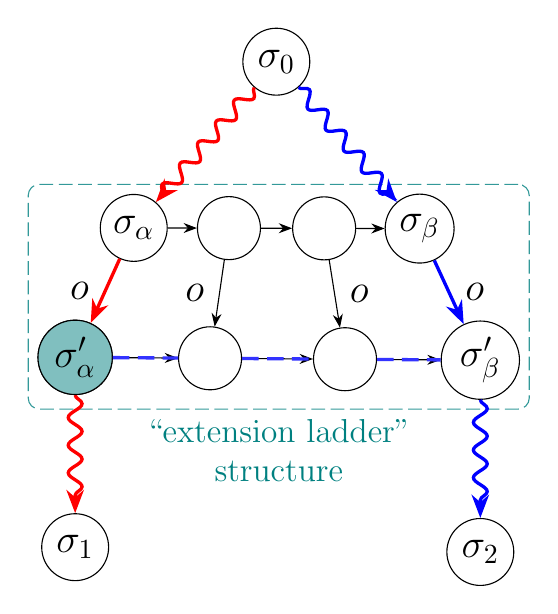
\begin{tikzpicture}
  \state{s0}{}{$\sigma_{0}$}
  \state{sa}{below left = 1.5*\vdist and 1.20*\hdist of s0}{$\sigma_{\alpha}$}
  \state{sa'}{below left = \vdist and 0.10*\hdist of sa}{$\sigma'_{\alpha}$}
  \state{s1}{below = 1.5*\vdist of sa'}{$\sigma_{1}$}

  \state{sb}{below right = 1.5*\vdist and 1.20*\hdist of s0}{$\sigma_{\beta}$}
  \state{sb'}{below right = \vdist and 0.10*\hdist of sb}{$\sigma'_{\beta}$}
  \state{s2}{below = 1.5*\vdist of sb'}{$\sigma_{2}$}

  \state{sx}{at = ($(sa.center)!0.333!(sb.center)$)}{}
  \state{sy}{at = ($(sa.center)!0.666!(sb.center)$)}{}
  \draw[edge] (sa) edge (sx) (sx) edge (sy) (sy) edge (sb);

  \state{sx'}{at = ($(sa'.center)!0.333!(sb'.center)$)}{}
  \state{sy'}{at = ($(sa'.center)!0.666!(sb'.center)$)}{}
  \draw[edge] (sa') edge (sx') (sx') edge (sy') (sy') edge (sb');

  \draw[edge] (sx) edge node[op, left = 2pt] {$o$} (sx') (sy) edge node[op, right = 2pt] {$o$} (sy');

  \draw (s0) edge[path, red, very thick] (sa) (sa) edge[edge, red, very thick] node[op, left = 2pt, black] {$o$} (sa') (sa') edge[path, red, very thick] (s1);
  \draw (s0) edge[path, blue, very thick] (sb) (sb) edge[edge, blue, very thick] node[op, right = 2pt, black] {$o$} (sb') (sb') edge[path, blue, very thick] (s2);

  \begin{pgfonlayer}{background}
	\node[fit = (sa) (sa') (sb) (sb'), rectangle, draw = teal!80, rounded corners, dash pattern = on 5pt off 2pt,
	  label = {[font = \large, align = center, teal] below:{``extension ladder'' \\ structure}}] {};
  \end{pgfonlayer}

  \state{}{at = (sa'), fill = teal!50}{$\sigma'_{\alpha}$}

  % sa' = LCA(s1, s2)
  \begin{scope}[conn/.style = {#1, very thick, dash pattern = on 6pt off 3pt}] 
	\draw[conn = {blue!80}] (sa') edge (sx') (sx') edge (sy') (sy') edge (sb');
  \end{scope}
\end{tikzpicture}
\end{document}
